%\captionsetup{width=0.9\textwidth,font=small}

As we now consider the oscillations between $R_1$ and $R_2$ as purely wide oscillations around the local minimum of $V_\text{int}$ at $R_2$, we are left with only two possible stable regimes in the overdamped case: either the molecule collapses to the origin, or a stable oscillation around $R_2$ is established. Focusing on the latter more interesting case, we recall the main result obtained in Section~\ref{oscillations:sec}, i.e.\\ that the driving frequency is the washboard frequency $\nu_\text{cm} = \frac{\Bar{v}_\text{cm}}{a}$. In addition, there is a relation between the external force $F$ and $\Bar{v}_\text{cm}$. In general, $\Bar{v}_\text{cm}$ grows when $F$ grows, but the exact dependence is non-trivial. In any case, we have an upper limit for the mean center-of-mass velocity, namely: $\Bar{v}_\text{cm} \leq F/m\gamma$. This means that the center of mass moves always more slowly than it would if it was not subject to any potential $V_\text{ext}$ or $V_\text{int}$. As we have previously mentioned, we observe that once the threshold value of $F$, for which a stable oscillation around $R_2$ is possible, is exceeded, the amplitude of such oscillation tends to decrease as $F$ and $\Bar{v}_\text{cm}$ increase. 

We now aim to study in a more rigorous way this trend, that might seem somewhat surprising. In fact, we expect to observe a peak in the amplitude of the oscillation when the washboard frequency approaches the natural oscillation frequency of the local minimum of $V_\text{int}$ at $R_2$. In the harmonic approximation this frequency is
\begin{equation}
   \nu_\text{harm} = \frac{\omega_\text{harm}}{2\pi} = \frac{1}{2\pi}\sqrt{\frac{V_\text{int}''(R_2)}{\mu}}.
   \label{eq:nu_harm}
\end{equation}

The evaluation of the second derivative of the internal potential at the minimum is straightforward and leads to

\begin{equation}
    V_\text{int}''(R_2) = 12U\left(R_2^4-R_1^2R_2^2 \right).
\end{equation}

To explore the possibility of resonances, we consider $R_1 = 1.5 a$ and $R_2 = 2.3 a$. We then change the external driving force $F$, and measure for each force the resulting peak-to-peak amplitude of the oscillations around $R_2$. We set $\gamma$ to $10 \g$, that is large enough to be in the overdamped case. The initial condition $R_0$ is set to $R_2$, in order to consistently trigger an oscillation around the minimum $R_2$, if possible. We then introduce the resonance velocity $v_\text{harm} = a\nu_\text{harm}$, for an easy comparison with $\Bar{v}_\text{cm}$. Figures~\ref{Fig:Resonance_a} and ~\ref{Fig:Resonance_b} report the oscillation amplitude obtained for a few values of $U$ (and therefore $\delta$ and $v_\text{harm}$). The black down-triangles in the plots represent the region before the depinning force, where the molecule does not move, and a blue circle marks an oscillation around $R_2$. In Fig.~\ref{Fig:Resonance_a}a, we see that for very small values of the potential barrier $\delta$, and thus of $v_\text{harm}$, once the oscillation is established, the amplitude decreases monotonically with $F$, in agreement with what was observed in Section~\ref{oscillations:sec}. In Fig.~\ref{Fig:Resonance_a} (c) and (d) we observe that when $\delta$ increases, a broad resonance peak appears. The peak becomes sharper and sharper as $U$ and thus $\delta$ increase, as reported in Fig.~\ref{Fig:Resonance_b}. Fig.~\ref{Fig:Resonance_5_b} is obtained with the same parameters as Fig.~\ref{Fig:Resonance_b}, but with a smaller damping factor $\gamma$. Here the resonance peaks are sharper, because the oscillator quality factor is larger~\cite{Mazzoldi}. %wikipedia https://en.wikipedia.org/wiki/Q_factor

\begin{figure}
\begin{center}
    \centering
    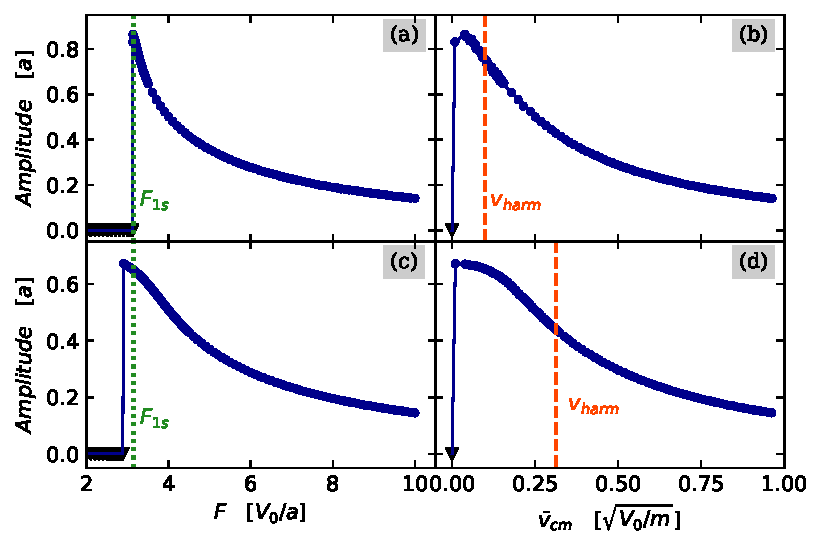
\includegraphics[width=1\linewidth]{Images/Resonance_2_a.pdf}
    \caption{The asymptotic oscillation amplitude $r_\text{max}-r_\text{min}$ as a function of \textbf{(a,c)} the applied force and \textbf{(b,d)} the resulting $\Bar{v}_\text{cm}$. The parameters are $R_1 = 1.5 a$, $R_2 = 2.3 a$, $\gamma = 10 \g$. The initial condition is $R_0=R_2$. The other parameters are: \textbf{(a,b)}: $U = 0.001 \p$ ($\delta = 1.4047 \times 10^{-2} V_0$); \textbf{(c,d)}: $U = 0.01 \p$ ($\delta = 0.14047 V_0$). The vertical dotted lines mark the static friction force $F_\text{1s}$ for one single free particle on $V_\text{ext}$. The vertical dashed lines mark the resonance velocities $v_\text{harm}$ corresponding to the harmonic frequencies for small amplitude oscillations near $R_2$. Panel \textbf{(b)}: $v_\text{harm} = 0.0989 \sqrt{V_0/m}$; panel \textbf{d}: $v_\text{harm} =  0.3127 \sqrt{V_0/m}$. The black triangles mark a value of $F$ below the depinning force, while the blue dots mark an oscillation around $R_2$. }
    \label{Fig:Resonance_a}
\end{center}
\end{figure}



\captionsetup{width=0.8\textwidth,font=normalsize}
\begin{figure}
\begin{center}
    \centering
    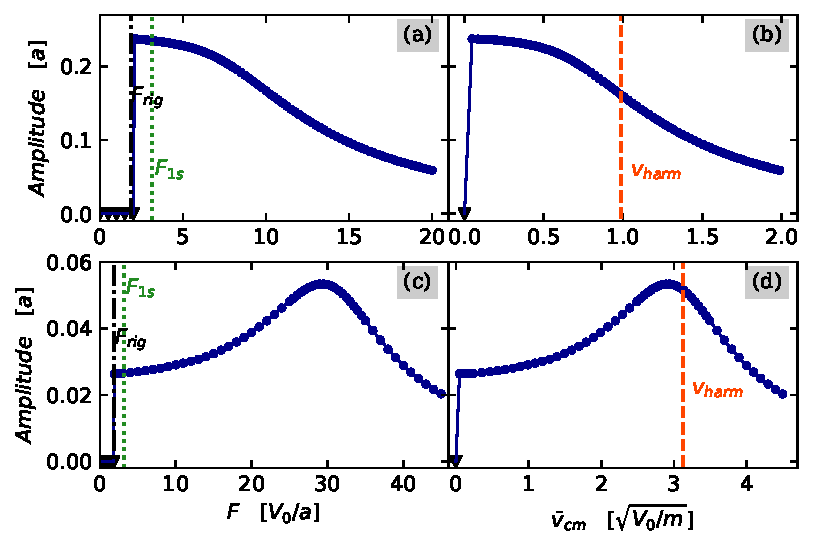
\includegraphics[width=0.85\linewidth]{Images/Resonance_2_b.pdf}
    \caption{Same as Fig.~\ref{Fig:Resonance_a}, but with stronger molecular potentials \textbf{(a,b)} $U = 0.1 \p$ ($\delta = 1.4047 \times 10^{-2} V_0$); \textbf{(c,d)} $U = 1 \p$ ($\delta = 14.047 V_0$). Panel \textbf{(b)}: $v_\text{harm} = 0.9888 \sqrt{V_0/m}$; panel \textbf{d}: $v_\text{harm} =  3.1267 \sqrt{V_0/m}$. The vertical dash-dotted lines mark the depinning force for a rigid molecule $F_\text{rig}$, where $r$ is fixed to $R_2$. }
    \label{Fig:Resonance_b}
\end{center}
\end{figure}


\begin{figure}
\begin{center}
    \centering
    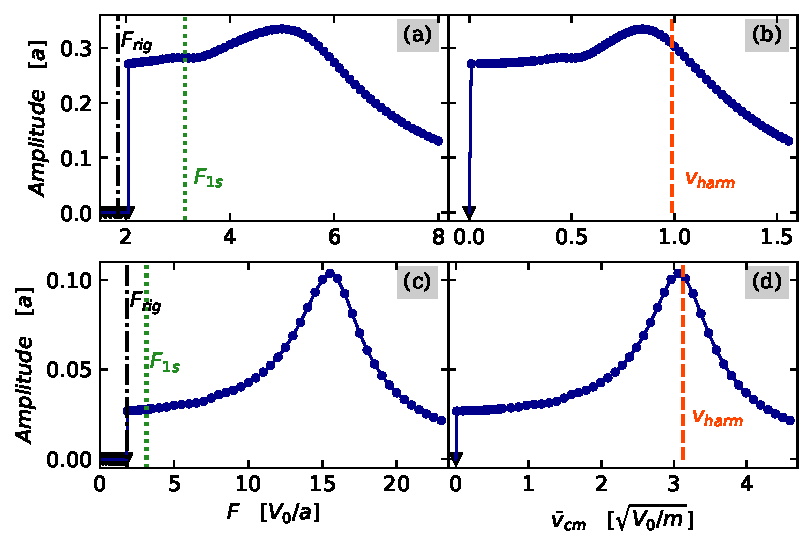
\includegraphics[width=0.85\linewidth]{Images/Resonance_b.pdf}
    \caption{Same as Fig.~\ref{Fig:Resonance_b}, but with $\gamma = 5 \g$}
    \label{Fig:Resonance_5_b}
\end{center}
\end{figure}


 

The picture is now clear: for small values of $\delta$, $V_\text{int}$ does not affect strongly the motion, the permitted oscillations around $R_2$ are wide, and a harmonic approximation of the phenomenon is meaningless. For increasing $\delta$, the forces generated by $V_\text{int}$ become stronger, the amplitude of the oscillations reduces and the harmonic approximation improves because the motion remains confined near the minimum.

For what concerns the value of the depinning force, we can see from Figs.~\ref{Fig:Resonance_a},~\ref{Fig:Resonance_b} and~\ref{Fig:Resonance_5_b}  (a,c) that it becomes smaller as $\delta$ increases. For very small $\delta$ the depinning force is almost the same as the static friction force for one free particle $F_\text{1s} = \pi \f$. When $\delta$ is larger, the depinning force decreases toward the depinning force for a rigid molecule where $r$ is fixed to $R_2$: $F_\text{rig} = \pi |\cos(\frac{\pi R_2}{a})| \f$. Clearly, $F_\text{rig} \leq F_\text{1s}$, so the bound exerted by $V_\text{int}$ helps the molecule to move on the external corrugated potential\footnote{A more exhaustive dissertation about the depinning force at various $U$ and $R_2$ can be found in Ref.~\cite{Cavallini}, \S~4.2.}.


\FloatBarrier
\subsection{Extra friction}

\begin{figure}
\begin{center}
    \centering
    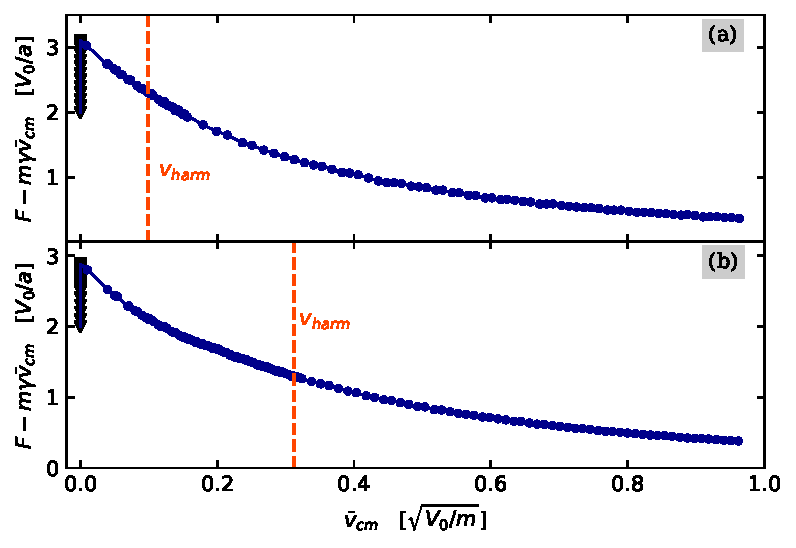
\includegraphics[width=1\linewidth]{Images/Attrito_2_a.pdf}
    \caption{Extra friction force for the molecule oscillating around $R_2$, as defined by Eq.~\eqref{eq:extra} as a function of the center-of-mass sliding velocity. \textbf{(a)} Same parameters as Fig.~\ref{Fig:Resonance_a} (a,b); \textbf{(b)} same parameters as Fig.~\ref{Fig:Resonance_a} (c,d).}
    \label{Fig:Attrito_a}
\end{center}
\end{figure}

\begin{figure}
\begin{center}
    \centering
    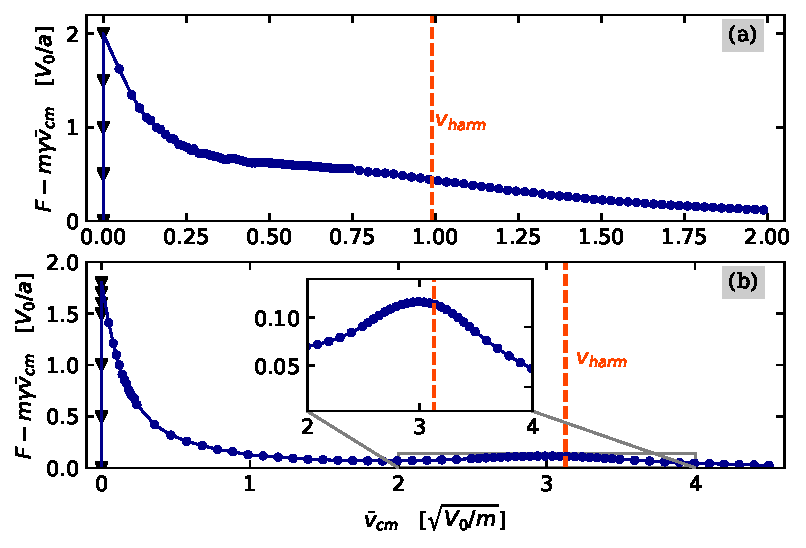
\includegraphics[width=1\linewidth]{Images/Attrito_2_b.pdf}
    \caption{Same as Fig.~\ref{Fig:Attrito_a} but: \textbf{(a)} same case as Fig.~\ref{Fig:Resonance_b} (a,b); \textbf{(b)} same case as Fig.~\ref{Fig:Resonance_b} (c,d).}
    \label{Fig:Attrito_b}
\end{center}
\end{figure}

\begin{figure}
\begin{center}
    \centering
    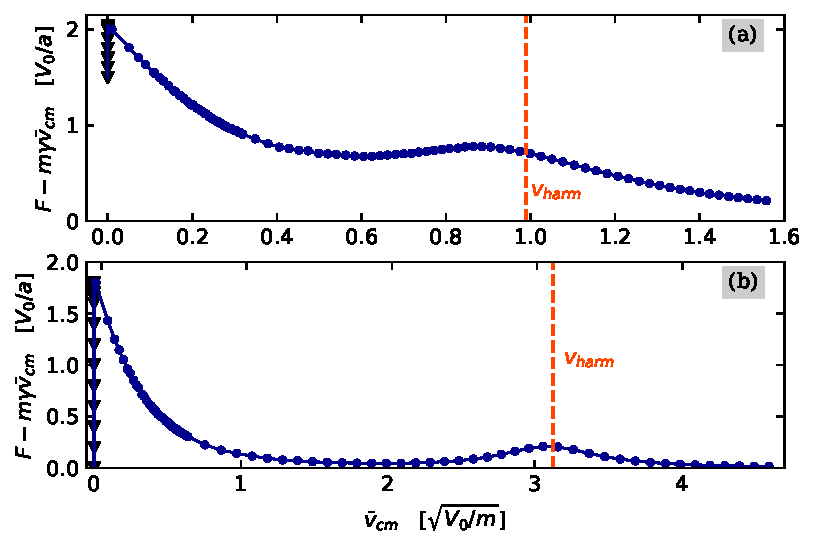
\includegraphics[width=1\linewidth]{Images/Attrito_b_2.pdf}
    \caption{Same as Fig.~\ref{Fig:Attrito_b} but wit $\gamma = 5 \g$.}
    \label{Fig:Attrito_5_b}
\end{center}
\end{figure}

We now aim to elucidate the extra friction, from now on abbreviated with e.f., originated from the molecule motions in a regime of steady advancement. We carry out a similar analysis as in Ref~\cite{Fusco} (where a pure harmonic molecular potential was adopted), adapting it to our model. We analyse the same oscillations studied in Figs.~\ref{Fig:Resonance_a} and~\ref{Fig:Resonance_b}, investigating how the e.f. varies with the strength of $V_\text{int}$. Figures~\ref{Fig:Attrito_a} and.~\ref{Fig:Attrito_b} report the e.f. force (per particle) that the molecule experience in addition to the trivial viscous friction force for a free particle in constant-velocity advancement at the same average velocity. The total average friction force exerted on the molecule (per particle) in a sliding scrolling regime, after the initial transient, is:

\begin{equation}
   \Bar{F}^{\text{tot}} = \frac{W^{\text{tot}}}{\Delta x} = \frac{1}{\Bar{v}_\text{cm}\tau} \int_{t_0}^{t_0+\tau}  F v_\text{cm}(t) dt =  \frac{F}{\Bar{v}_\text{cm}\tau} \int_{t_0}^{t_0+\tau}  v_\text{cm}(t) dt = F,
   \label{eq:tot}
\end{equation}
where $F$ is the force acting on one particle, $\Delta x = \Bar{v}_\text{cm}\tau$ is the total advancement path, $\int_{t_0}^{t_0+\tau}  v_\text{cm}(t) dt = \Bar{v}_\text{cm}\tau$ defines the average velocity, and $\tau$ is an integer number f periods of oscillation of the internal coordinate $r$. Recalling that a free particle pulled by a constant force $F$ moves with a terminal velocity $v_\text{cm}(t) = v_\text{free} = F/m\gamma $, the trivial friction force due to the free motion of the molecule (per particle) is:

\begin{equation}
   \Bar{F}^{\text{free}} = m \gamma \Bar{v}_\text{cm}.
   \label{eq:free}
\end{equation}

The extra friction force per particle is then
\begin{equation}
   \Bar{F}^{\text{extra}} = F - m\gamma \Bar{v}_\text{cm} = m\gamma (v_\text{free}-\Bar{v}_\text{cm}),
   \label{eq:extra}
\end{equation}
indicating that it measures the slowing down due to accelerations and decelerations of the center of mass and due to internal motions.

Figures.~\ref{Fig:Attrito_a} and~\ref{Fig:Attrito_b} report also the range where $F$ is insufficient to win the static friction, leading to $\Bar{v}_\text{cm} = 0$ (black down-triangles): here the molecule does not move, and Eqs.~\eqref{eq:tot} and~\eqref{eq:free} do not apply. After the depinning force, as long as the molecule starts to move, the e.f. is maximum, and then it decreases as the driving force force, and thus the sliding speed, increases. In the limit of large $F$, $\Bar{v}_\text{cm} \sim{\frac{F}{m\gamma}} $, i.e.\ for strong external force the perturbation induced by $V_\text{ext}$ and $V_\text{int}$ tends to become negligible, and the motion of the center of mass resembles that of a free particle.

In Fig.~\ref{Fig:Attrito_a}a, where $\delta = 1.4047 \times 10^{-2} V_0$, the e.f.\ decreases monotonically. Also in Fig.~\ref{Fig:Attrito_a}b, for a larger $\delta = 0.14047 V_0$, the e.f.\ decreases monotonically, but a very weak shoulder is observed for $\Bar{v}_\text{cm}$ near the harmonic velocity $v_\text{harm}$. This shoulder corresponds to the amplitude shoulder already reported in Fig.~\ref{Fig:Resonance_a}d. In Fig.~\ref{Fig:Attrito_b}b a proper peak in friction becomes visible as $\nu_\text{harm}$ increases. The friction peak is obviously related to the resonance peak in Fig.~\ref{Fig:Resonance_b}d. The peaks becomes again sharper when $\gamma$ is decreased, as reported in Fig.~\ref{Fig:Attrito_5_b}.

The physical explanation is simple: for increasing $\delta$ the amplitude of the oscillation reduces, the harmonic approximation becomes better and better and we observe an amplitude resonance peak when the frequency of the effective driving force approaches the natural oscillation frequency of $V_\text{int}$ around $R_2$. This peak in the amplitude of the oscillations induces a peak in the e.f. because part of the energy pumped into the molecule by $F$ is spent to sustain the motion of the relative coordinate $r$. We can also notice that $\Bar{F}^{\text{extra}}$ becomes generally smaller for larger $\delta$, again due to the amplitude of the $r$ oscillations decreasing with increasing rigidity of the molecule.

Eventually we recover the results obtained with a pure harmonic potential in Ref.~\cite{Fusco}, when we analyze oscillations around $R_2$ in the limit of small harmonic displacements. Our system is however more complex, because the harmonic approximation is valid only for quite large values of $V_\text{int}$, when the motion remains restricted to a small region around $R_2$. 